\documentclass[tikz,border=4pt]{standalone}
\usepackage{ctex}
\usepackage{pgfplots}
\pgfplotsset{compat=1.18}
\begin{document}
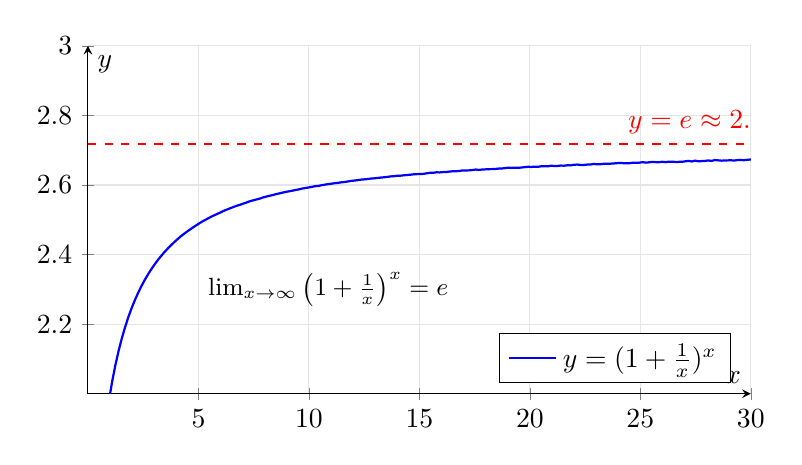
\begin{tikzpicture}
\begin{axis}[
    axis lines=middle, width=10cm, height=6cm,
    xmin=0, xmax=30, ymin=2, ymax=3,
    xlabel={$x$}, ylabel={$y$},
    samples=200, grid=both, grid style={gray!20},
    legend pos=south east,
]
\addplot[blue, thick, domain=0.5:30] {(1 + 1/x)^x};
\addlegendentry{$y=(1+\frac{1}{x})^x$}
\draw[red, thick, dashed] (axis cs:0,2.71828) -- (axis cs:30,2.71828);
\node[red, anchor=west] at (axis cs:24, 2.78) {$y=e\approx 2.718$};
\node[anchor=west] at (axis cs:5, 2.3) {\small $\lim_{x\to\infty}\left(1+\frac{1}{x}\right)^x = e$};
\end{axis}
\end{tikzpicture}
\end{document}
